% Options for packages loaded elsewhere
\PassOptionsToPackage{unicode}{hyperref}
\PassOptionsToPackage{hyphens}{url}
\PassOptionsToPackage{dvipsnames,svgnames,x11names}{xcolor}
%
\documentclass[
  letterpaper,
  DIV=11,
  numbers=noendperiod]{scrartcl}

\usepackage{amsmath,amssymb}
\usepackage{iftex}
\ifPDFTeX
  \usepackage[T1]{fontenc}
  \usepackage[utf8]{inputenc}
  \usepackage{textcomp} % provide euro and other symbols
\else % if luatex or xetex
  \usepackage{unicode-math}
  \defaultfontfeatures{Scale=MatchLowercase}
  \defaultfontfeatures[\rmfamily]{Ligatures=TeX,Scale=1}
\fi
\usepackage{lmodern}
\ifPDFTeX\else  
    % xetex/luatex font selection
\fi
% Use upquote if available, for straight quotes in verbatim environments
\IfFileExists{upquote.sty}{\usepackage{upquote}}{}
\IfFileExists{microtype.sty}{% use microtype if available
  \usepackage[]{microtype}
  \UseMicrotypeSet[protrusion]{basicmath} % disable protrusion for tt fonts
}{}
\makeatletter
\@ifundefined{KOMAClassName}{% if non-KOMA class
  \IfFileExists{parskip.sty}{%
    \usepackage{parskip}
  }{% else
    \setlength{\parindent}{0pt}
    \setlength{\parskip}{6pt plus 2pt minus 1pt}}
}{% if KOMA class
  \KOMAoptions{parskip=half}}
\makeatother
\usepackage{xcolor}
\setlength{\emergencystretch}{3em} % prevent overfull lines
\setcounter{secnumdepth}{-\maxdimen} % remove section numbering
% Make \paragraph and \subparagraph free-standing
\ifx\paragraph\undefined\else
  \let\oldparagraph\paragraph
  \renewcommand{\paragraph}[1]{\oldparagraph{#1}\mbox{}}
\fi
\ifx\subparagraph\undefined\else
  \let\oldsubparagraph\subparagraph
  \renewcommand{\subparagraph}[1]{\oldsubparagraph{#1}\mbox{}}
\fi


\providecommand{\tightlist}{%
  \setlength{\itemsep}{0pt}\setlength{\parskip}{0pt}}\usepackage{longtable,booktabs,array}
\usepackage{calc} % for calculating minipage widths
% Correct order of tables after \paragraph or \subparagraph
\usepackage{etoolbox}
\makeatletter
\patchcmd\longtable{\par}{\if@noskipsec\mbox{}\fi\par}{}{}
\makeatother
% Allow footnotes in longtable head/foot
\IfFileExists{footnotehyper.sty}{\usepackage{footnotehyper}}{\usepackage{footnote}}
\makesavenoteenv{longtable}
\usepackage{graphicx}
\makeatletter
\def\maxwidth{\ifdim\Gin@nat@width>\linewidth\linewidth\else\Gin@nat@width\fi}
\def\maxheight{\ifdim\Gin@nat@height>\textheight\textheight\else\Gin@nat@height\fi}
\makeatother
% Scale images if necessary, so that they will not overflow the page
% margins by default, and it is still possible to overwrite the defaults
% using explicit options in \includegraphics[width, height, ...]{}
\setkeys{Gin}{width=\maxwidth,height=\maxheight,keepaspectratio}
% Set default figure placement to htbp
\makeatletter
\def\fps@figure{htbp}
\makeatother

\KOMAoption{captions}{tableheading}
\makeatletter
\makeatother
\makeatletter
\makeatother
\makeatletter
\@ifpackageloaded{caption}{}{\usepackage{caption}}
\AtBeginDocument{%
\ifdefined\contentsname
  \renewcommand*\contentsname{Table of contents}
\else
  \newcommand\contentsname{Table of contents}
\fi
\ifdefined\listfigurename
  \renewcommand*\listfigurename{List of Figures}
\else
  \newcommand\listfigurename{List of Figures}
\fi
\ifdefined\listtablename
  \renewcommand*\listtablename{List of Tables}
\else
  \newcommand\listtablename{List of Tables}
\fi
\ifdefined\figurename
  \renewcommand*\figurename{Figure}
\else
  \newcommand\figurename{Figure}
\fi
\ifdefined\tablename
  \renewcommand*\tablename{Table}
\else
  \newcommand\tablename{Table}
\fi
}
\@ifpackageloaded{float}{}{\usepackage{float}}
\floatstyle{ruled}
\@ifundefined{c@chapter}{\newfloat{codelisting}{h}{lop}}{\newfloat{codelisting}{h}{lop}[chapter]}
\floatname{codelisting}{Listing}
\newcommand*\listoflistings{\listof{codelisting}{List of Listings}}
\makeatother
\makeatletter
\@ifpackageloaded{caption}{}{\usepackage{caption}}
\@ifpackageloaded{subcaption}{}{\usepackage{subcaption}}
\makeatother
\makeatletter
\@ifpackageloaded{tcolorbox}{}{\usepackage[skins,breakable]{tcolorbox}}
\makeatother
\makeatletter
\@ifundefined{shadecolor}{\definecolor{shadecolor}{rgb}{.97, .97, .97}}
\makeatother
\makeatletter
\makeatother
\makeatletter
\makeatother
\ifLuaTeX
  \usepackage{selnolig}  % disable illegal ligatures
\fi
\IfFileExists{bookmark.sty}{\usepackage{bookmark}}{\usepackage{hyperref}}
\IfFileExists{xurl.sty}{\usepackage{xurl}}{} % add URL line breaks if available
\urlstyle{same} % disable monospaced font for URLs
\hypersetup{
  pdftitle={Water for Good},
  colorlinks=true,
  linkcolor={blue},
  filecolor={Maroon},
  citecolor={Blue},
  urlcolor={Blue},
  pdfcreator={LaTeX via pandoc}}

\title{Water for Good}
\usepackage{etoolbox}
\makeatletter
\providecommand{\subtitle}[1]{% add subtitle to \maketitle
  \apptocmd{\@title}{\par {\large #1 \par}}{}{}
}
\makeatother
\subtitle{Report}
\author{}
\date{}

\begin{document}
\maketitle
\ifdefined\Shaded\renewenvironment{Shaded}{\begin{tcolorbox}[interior hidden, boxrule=0pt, breakable, frame hidden, enhanced, borderline west={3pt}{0pt}{shadecolor}, sharp corners]}{\end{tcolorbox}}\fi

\textbf{Uni-variate EDA}

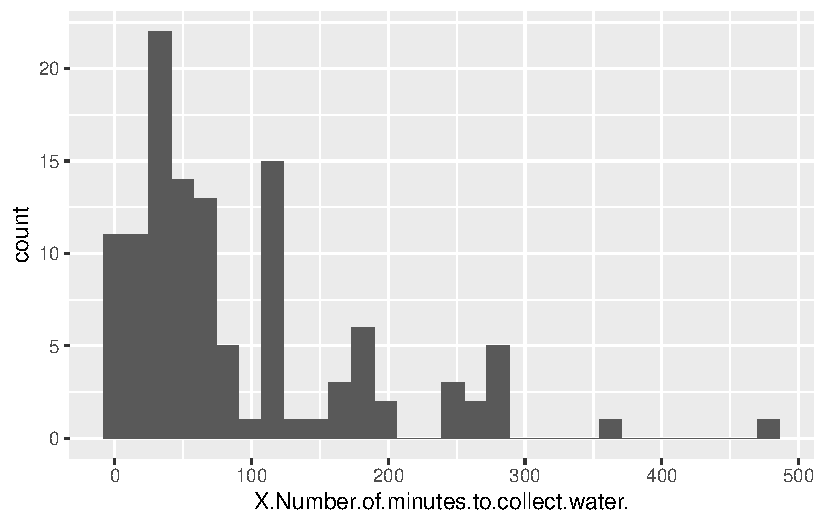
\includegraphics{report_files/figure-pdf/unnamed-chunk-3-1.pdf}

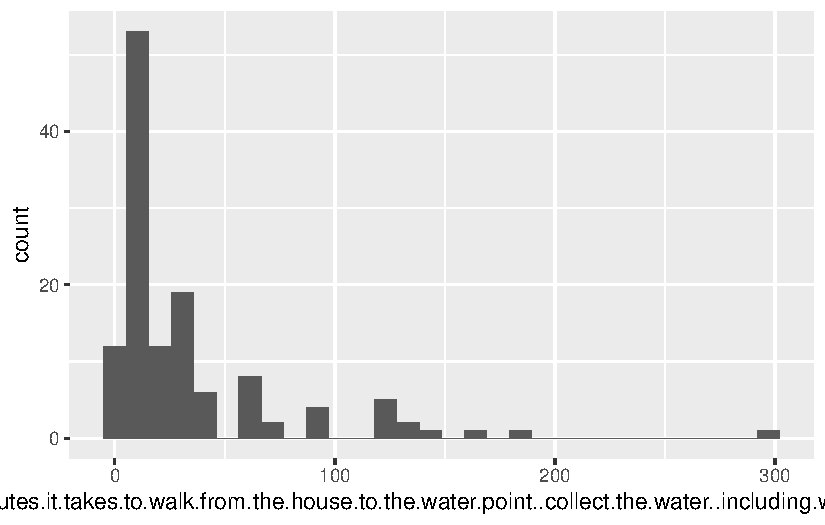
\includegraphics{report_files/figure-pdf/unnamed-chunk-4-1.pdf}

\begin{verbatim}
# A tibble: 1 x 8
  n_missing numeric.mean numeric.sd numeric.p0 numeric.p25 numeric.p50
      <int>        <dbl>      <dbl>      <dbl>       <dbl>       <dbl>
1        11         88.4       88.0          2          30          60
  numeric.p75 numeric.p100
        <dbl>        <dbl>
1         120          480
\end{verbatim}

\begin{verbatim}
# A tibble: 1 x 8
  n_missing numeric.mean numeric.sd numeric.p0 numeric.p25 numeric.p50
      <int>        <dbl>      <dbl>      <dbl>       <dbl>       <dbl>
1         1         34.7       43.1          3          10          15
  numeric.p75 numeric.p100
        <dbl>        <dbl>
1          35          300
\end{verbatim}

Both datasets are clearly right skewed therefore using the median amount
of time for water collection drastically decreased from the baseline to
the recent project survey. The median amount of time for water
collection decreased from about 60 to 15 minutes. With the ranges also
being drastically smaller for the minutes for the post survey.

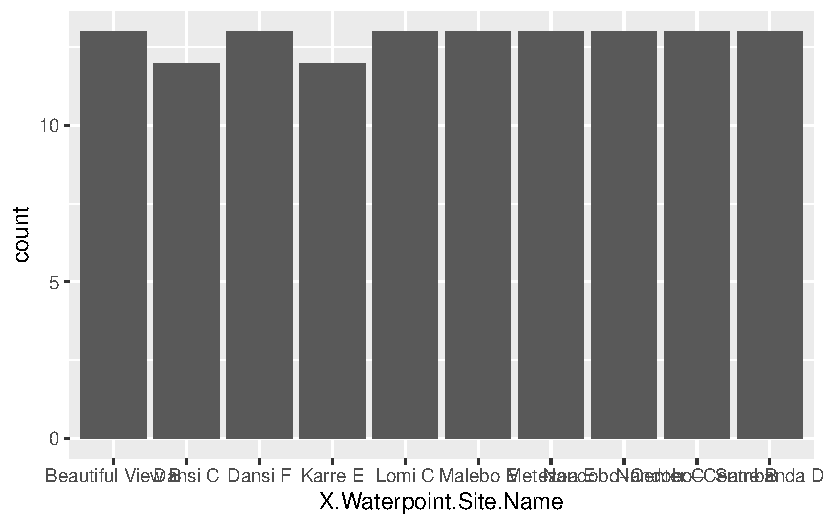
\includegraphics{report_files/figure-pdf/unnamed-chunk-7-1.pdf}

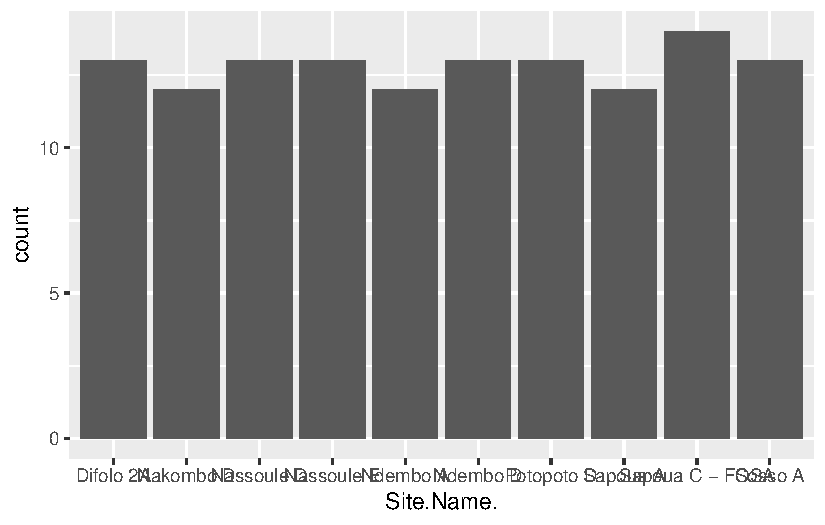
\includegraphics{report_files/figure-pdf/unnamed-chunk-8-1.pdf}

Based of the both the graphs, there is no overlap in the waterpoint site
names. Having a project and baseline, wondering if there is any other
data that would help keep one dataset as a base for comparison.

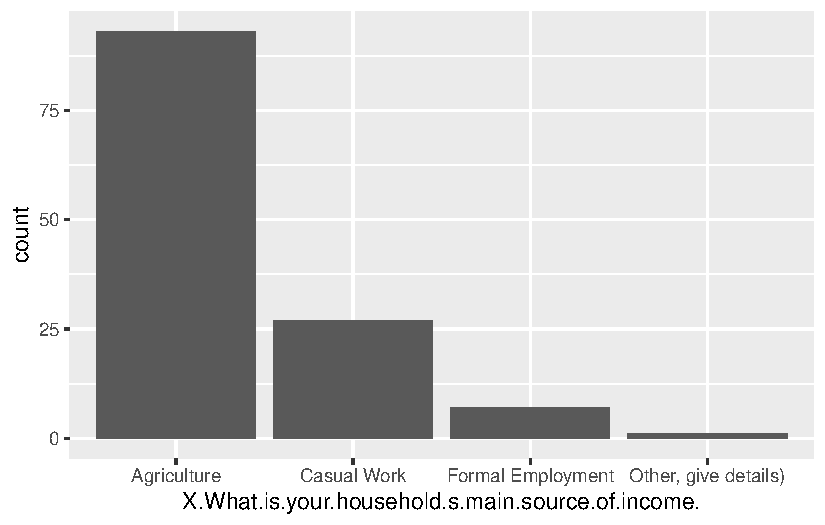
\includegraphics{report_files/figure-pdf/unnamed-chunk-9-1.pdf}

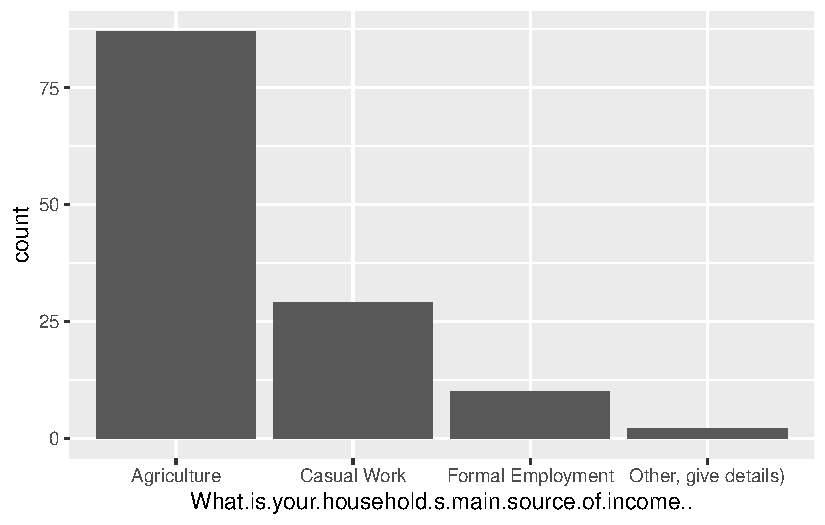
\includegraphics{report_files/figure-pdf/unnamed-chunk-10-1.pdf}

Both have similar household income levels, this could be used a baseline
of comparison rather than the waterpoint site name.

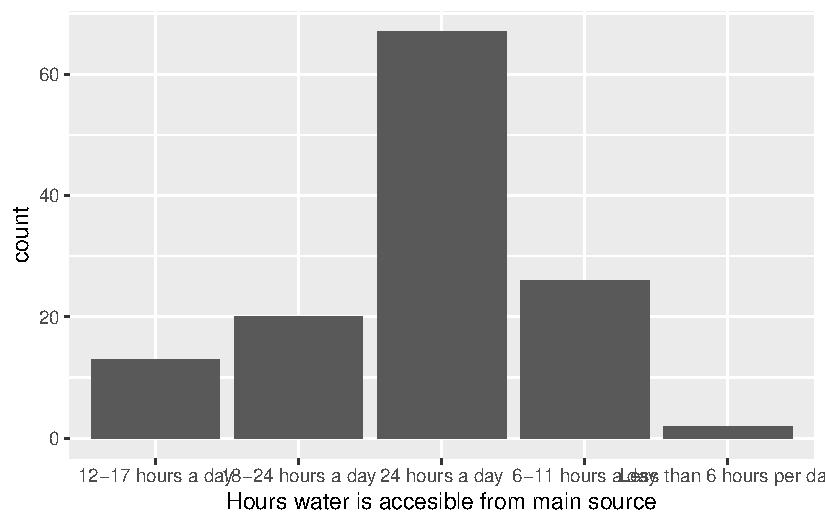
\includegraphics{report_files/figure-pdf/unnamed-chunk-11-1.pdf}

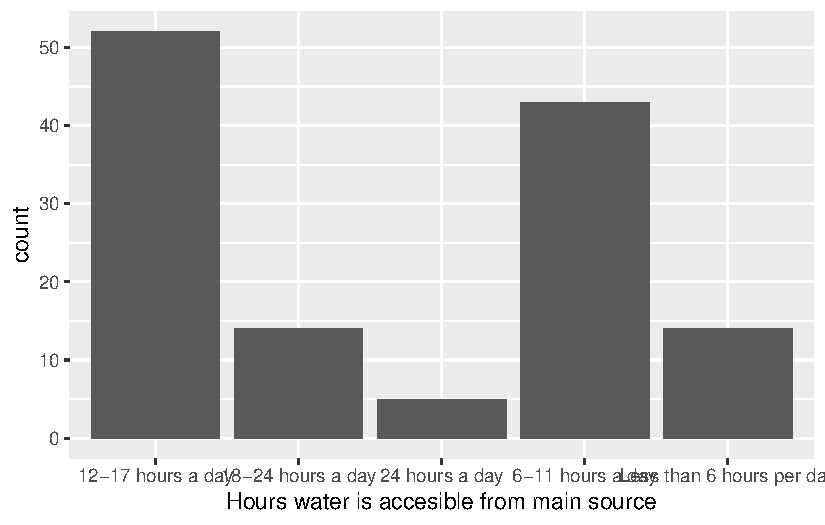
\includegraphics{report_files/figure-pdf/unnamed-chunk-12-1.pdf}

Based on both the graphs, there is a increase in the ``12-17 hours a
day'' water availability post the baseline survey. However, an
interesting thing that the 24 hours a day drastically decreased from
around 65 to 5 wells available.

\hypertarget{bi-variate-eda}{%
\paragraph{Bi-variate EDA}\label{bi-variate-eda}}

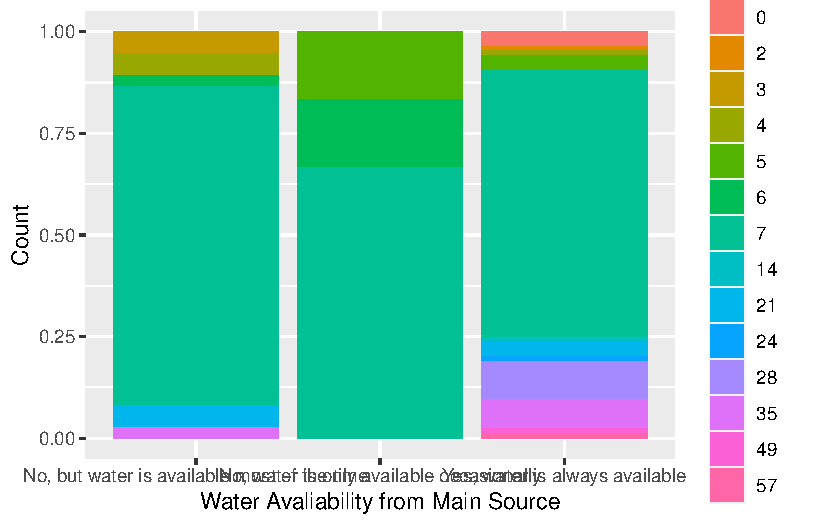
\includegraphics{report_files/figure-pdf/unnamed-chunk-13-1.pdf}

For the instances that water is always available, there seems to be a
higher percentage of more trips taken to the main water source. One
thing that did stand out to me was the response of ``No, but water is
available most of the time'' had the most amount of ``medium'' trips
taken (around 5-6 trips). Assuming that they had bigger containers to
store and carry water, therefore needing less trips. The people who have
constant water access, have smaller containers and therefore make more
trips in order to obtain water from their main water source.

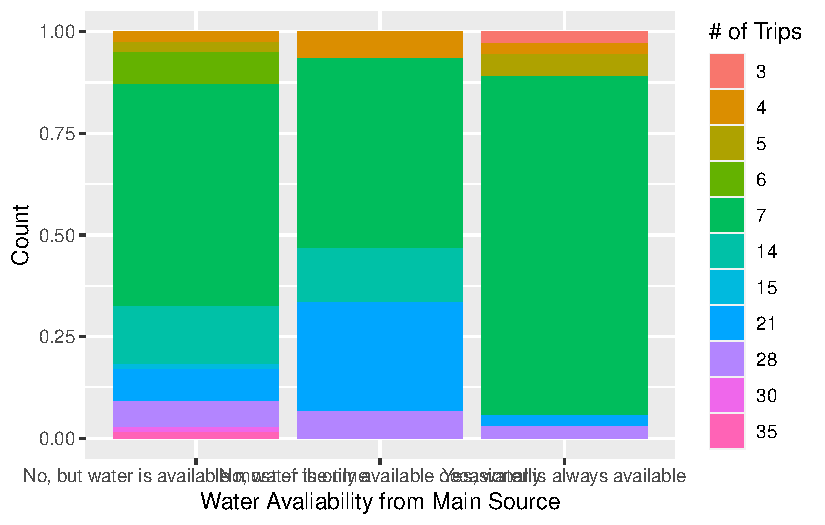
\includegraphics{report_files/figure-pdf/unnamed-chunk-14-1.pdf}

We see a drastic difference in the ``Yes, water is always available''
column as the number of trips frequented dropped from a high of 24-57
trips to a majority of only 6-7 trips. Assuming the project survey was
done months after the wells were drilled, we could see that it helped in
reducing the trips made by local residents.

\hypertarget{linear-regression-and-hypothesis-testing}{%
\paragraph{Linear Regression and Hypothesis
Testing}\label{linear-regression-and-hypothesis-testing}}

\begin{longtable}[]{@{}
  >{\raggedright\arraybackslash}p{(\columnwidth - 8\tabcolsep) * \real{0.6022}}
  >{\raggedleft\arraybackslash}p{(\columnwidth - 8\tabcolsep) * \real{0.0968}}
  >{\raggedleft\arraybackslash}p{(\columnwidth - 8\tabcolsep) * \real{0.1075}}
  >{\raggedleft\arraybackslash}p{(\columnwidth - 8\tabcolsep) * \real{0.1075}}
  >{\raggedleft\arraybackslash}p{(\columnwidth - 8\tabcolsep) * \real{0.0860}}@{}}
\toprule\noalign{}
\begin{minipage}[b]{\linewidth}\raggedright
term
\end{minipage} & \begin{minipage}[b]{\linewidth}\raggedleft
estimate
\end{minipage} & \begin{minipage}[b]{\linewidth}\raggedleft
std.error
\end{minipage} & \begin{minipage}[b]{\linewidth}\raggedleft
statistic
\end{minipage} & \begin{minipage}[b]{\linewidth}\raggedleft
p.value
\end{minipage} \\
\midrule\noalign{}
\endhead
\bottomrule\noalign{}
\endlastfoot
(Intercept) & 13.546 & 1.267 & 10.689 & 0.000 \\
Is.water.always.available.from.your.main.water.source.. & -2.798 & 0.964
& -2.901 & 0.004 \\
\end{longtable}

\begin{verbatim}
# A tibble: 2 x 2
  term                                                    p_value
  <chr>                                                     <dbl>
1 Is.water.always.available.from.your.main.water.source..   0.006
2 intercept                                                 0.006
\end{verbatim}

\(Trips = 13.546 - 2.798*Water\_availability\)

Where

No, water is only available occasionally = 0, No, but water is available
most of the time = 1

Yes, water is always available = 2

Since p-value is lower than 0.05, we can reject the null hypothesis and
conclude that there is a statistically linear relationship between water
availability from the waterpoint and number of trips taken. Therefore,
whenever there are more water availability from the waterpoint site, the
less number of trips taken.

\hypertarget{summary-statistics}{%
\subsubsection{Summary Statistics}\label{summary-statistics}}

\hypertarget{counts-by-gender}{%
\paragraph{Counts by Gender}\label{counts-by-gender}}

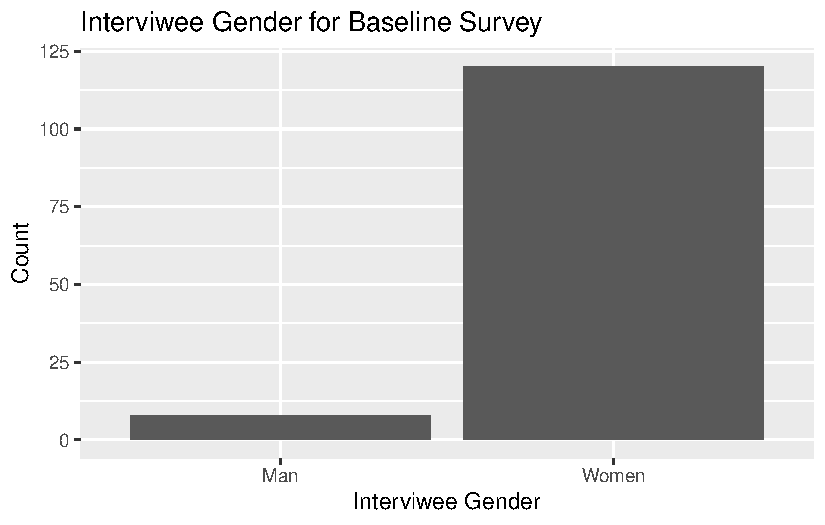
\includegraphics{report_files/figure-pdf/unnamed-chunk-16-1.pdf}

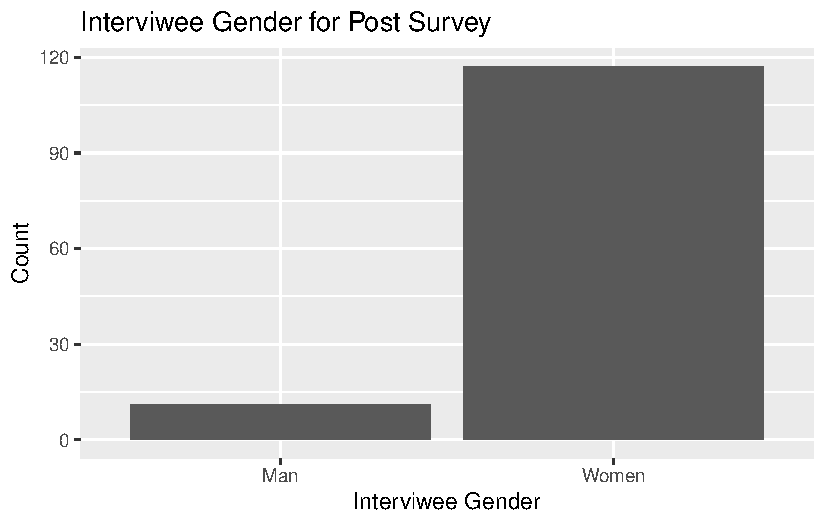
\includegraphics{report_files/figure-pdf/unnamed-chunk-17-1.pdf}

Both baseline and project survey results have similar demographics.

\hypertarget{counts-by-education-level}{%
\paragraph{Counts by Education Level}\label{counts-by-education-level}}

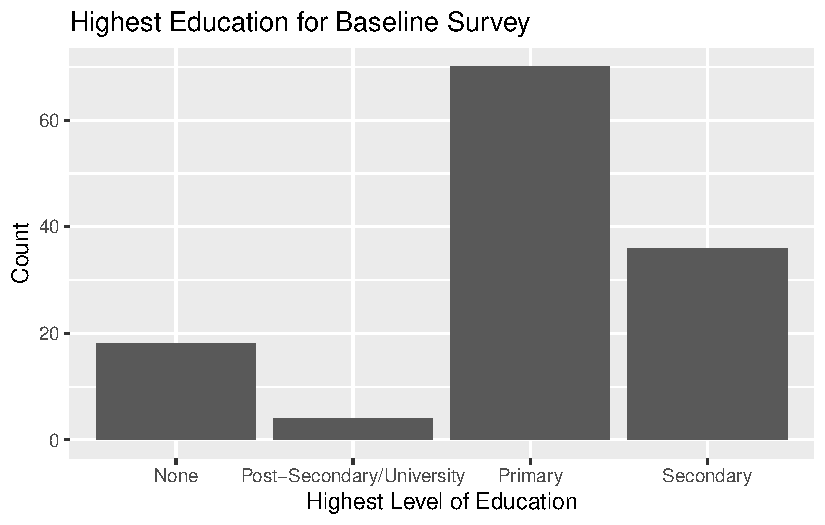
\includegraphics{report_files/figure-pdf/unnamed-chunk-18-1.pdf}

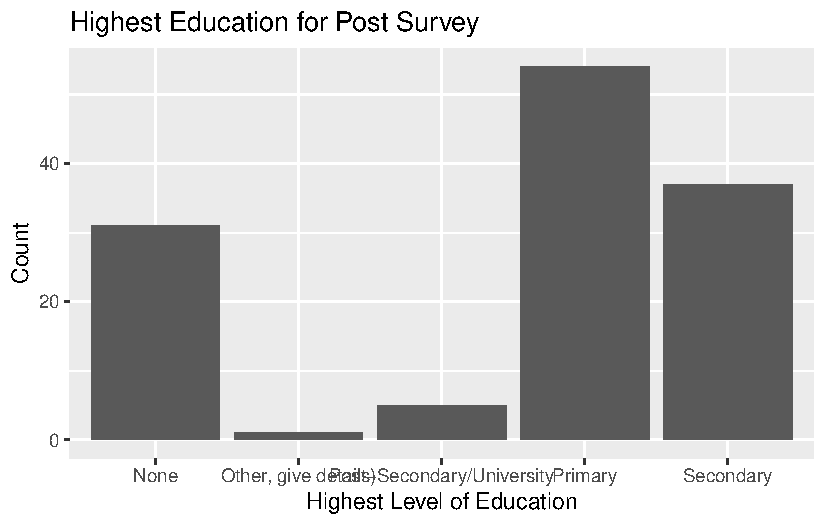
\includegraphics{report_files/figure-pdf/unnamed-chunk-19-1.pdf}

\begin{verbatim}
# A tibble: 4 x 2
  X.What.is.the.highest.level.of.education.obtained.by.the.head.of.the.h~1 count
  <chr>                                                                    <int>
1 None                                                                        18
2 Post-Secondary/University                                                    4
3 Primary                                                                     70
4 Secondary                                                                   36
# i abbreviated name:
#   1: X.What.is.the.highest.level.of.education.obtained.by.the.head.of.the.household.
\end{verbatim}

\begin{verbatim}
# A tibble: 5 x 2
  What.is.the.highest.level.of.education.attained.by.the.head.of.the.hou~1 count
  <chr>                                                                    <int>
1 None                                                                        31
2 Other, give details)                                                         1
3 Post-Secondary/University                                                    5
4 Primary                                                                     54
5 Secondary                                                                   37
# i abbreviated name:
#   1: What.is.the.highest.level.of.education.attained.by.the.head.of.the.household..
\end{verbatim}

Both surveys had the same number of participants, 128. Baseline Survey
had more people who completed primary school, but the rest of the
distribution regarding secondary, post secondary and other remained the
same.

\hypertarget{counts-by-household-income}{%
\paragraph{Counts by household
income}\label{counts-by-household-income}}

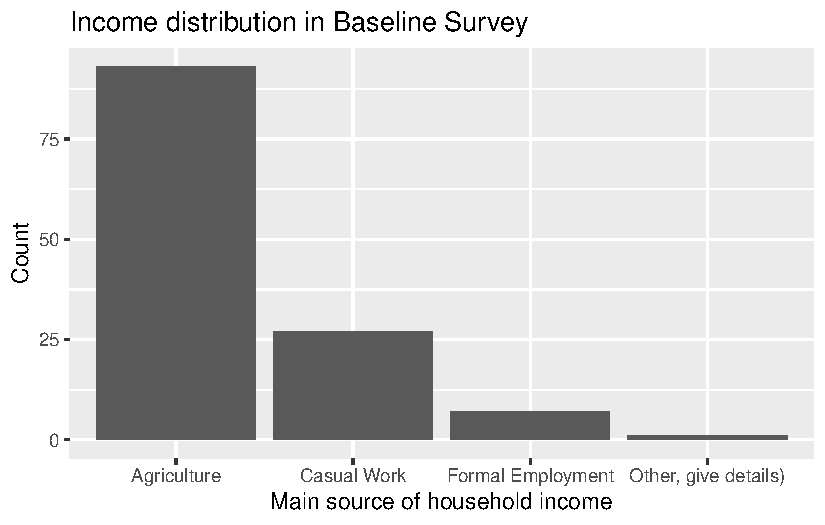
\includegraphics{report_files/figure-pdf/unnamed-chunk-21-1.pdf}

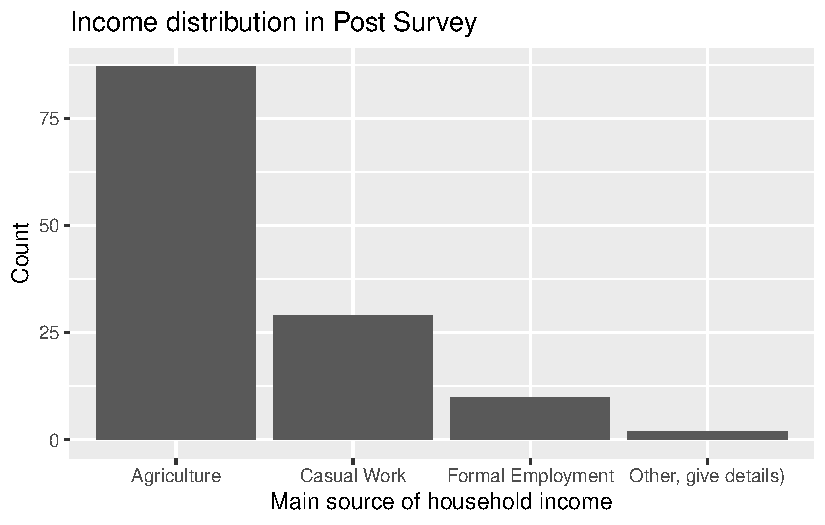
\includegraphics{report_files/figure-pdf/unnamed-chunk-22-1.pdf}

Similar distributions in Income distribution in both baseline and post
survey.

\hypertarget{average-number-of-people-living-in-household}{%
\paragraph{Average number of people living in
household}\label{average-number-of-people-living-in-household}}

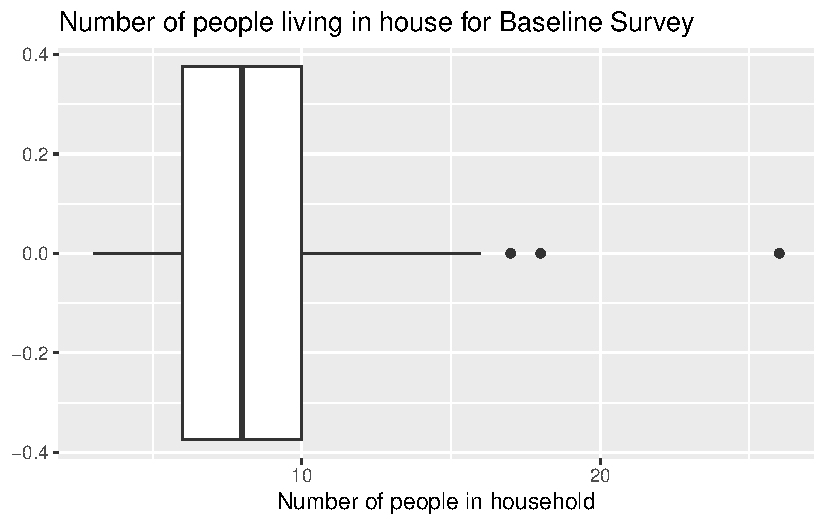
\includegraphics{report_files/figure-pdf/unnamed-chunk-23-1.pdf}

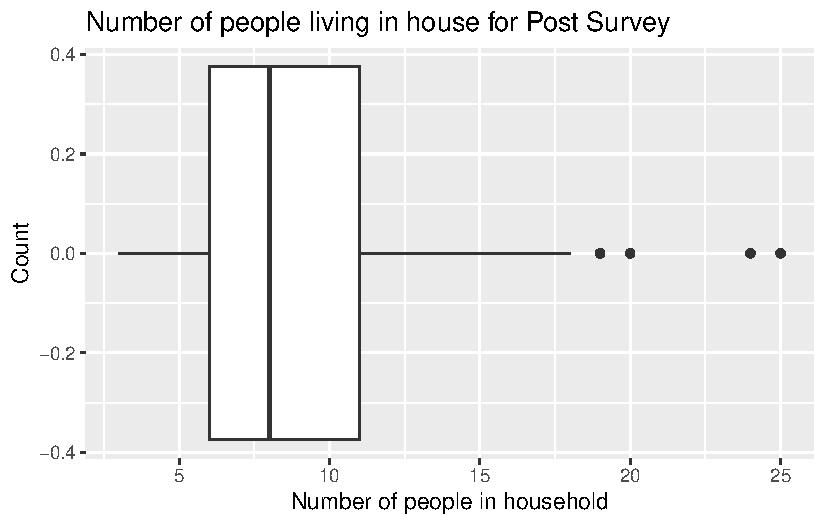
\includegraphics{report_files/figure-pdf/unnamed-chunk-24-1.pdf}

\begin{verbatim}
# A tibble: 17 x 2
   X.How.many.people.live.in.your.household.in.total..including.yourself. count
                                                                    <int> <int>
 1                                                                      3     3
 2                                                                      4     5
 3                                                                      5    14
 4                                                                      6    19
 5                                                                      7    21
 6                                                                      8    13
 7                                                                      9    12
 8                                                                     10    10
 9                                                                     11     8
10                                                                     12     9
11                                                                     13     2
12                                                                     14     5
13                                                                     15     2
14                                                                     16     1
15                                                                     17     1
16                                                                     18     2
17                                                                     26     1
\end{verbatim}

\begin{verbatim}
# A tibble: 19 x 2
   How.many.people.live.in.your.household.in.total..Ie.the.number.of.peo~1 count
                                                                     <int> <int>
 1                                                                       3     5
 2                                                                       4    10
 3                                                                       5    12
 4                                                                       6    16
 5                                                                       7    17
 6                                                                       8    13
 7                                                                       9     6
 8                                                                      10    15
 9                                                                      11     3
10                                                                      12     8
11                                                                      13     4
12                                                                      14     1
13                                                                      15     8
14                                                                      17     3
15                                                                      18     1
16                                                                      19     1
17                                                                      20     3
18                                                                      24     1
19                                                                      25     1
# i abbreviated name:
#   1: How.many.people.live.in.your.household.in.total..Ie.the.number.of.people.living.under.this.roof..including.yourself..
\end{verbatim}

Similar distribution for both baseline and project.

\hypertarget{waterpoint-site-name}{%
\paragraph{Waterpoint Site Name}\label{waterpoint-site-name}}

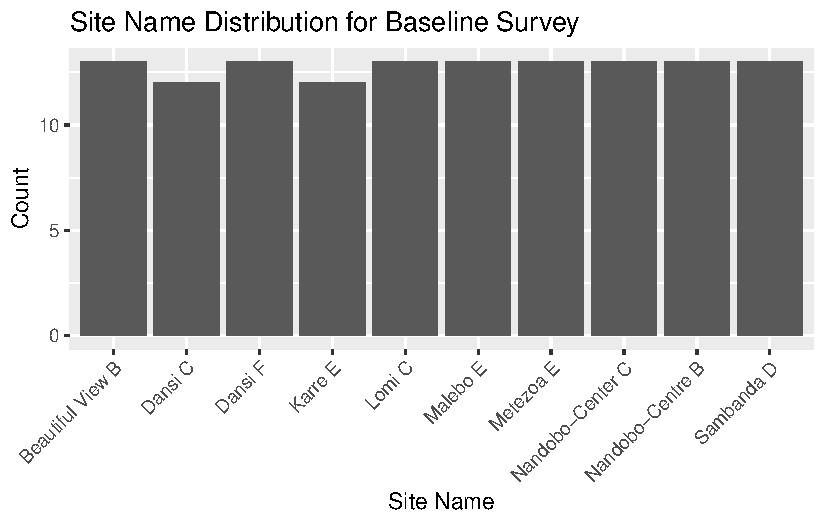
\includegraphics{report_files/figure-pdf/unnamed-chunk-26-1.pdf}

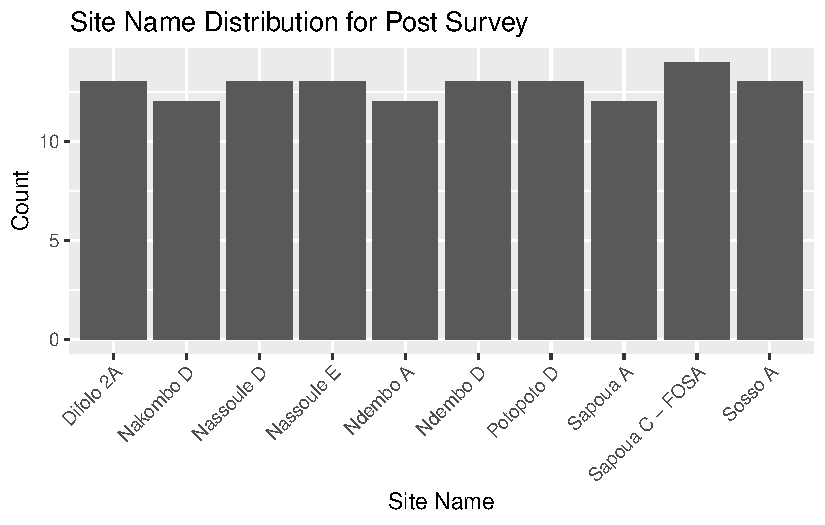
\includegraphics{report_files/figure-pdf/unnamed-chunk-27-1.pdf}

We can clearly see that baseline and project had different waterpoint
site name. Difference between them suggests possibly not the best to
compare rather create summary statistics for both surveys individually.

\hypertarget{subjects-within-prefecture}{%
\paragraph{Subjects within
Prefecture}\label{subjects-within-prefecture}}

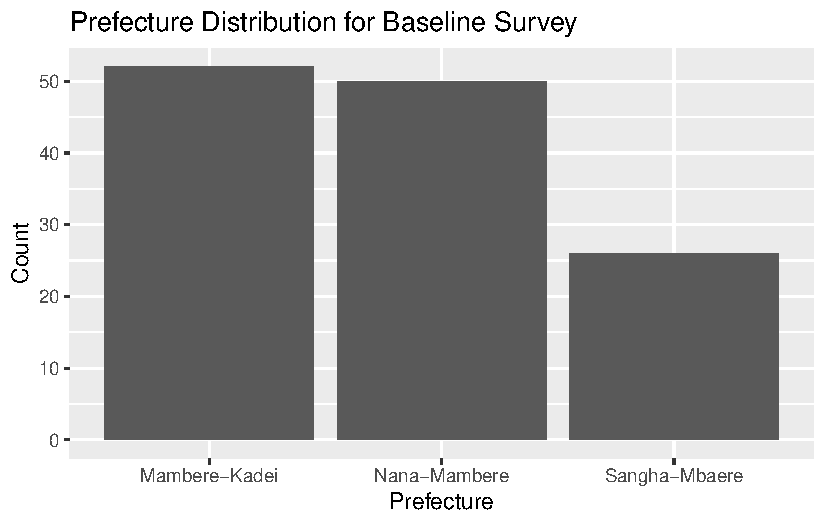
\includegraphics{report_files/figure-pdf/unnamed-chunk-28-1.pdf}

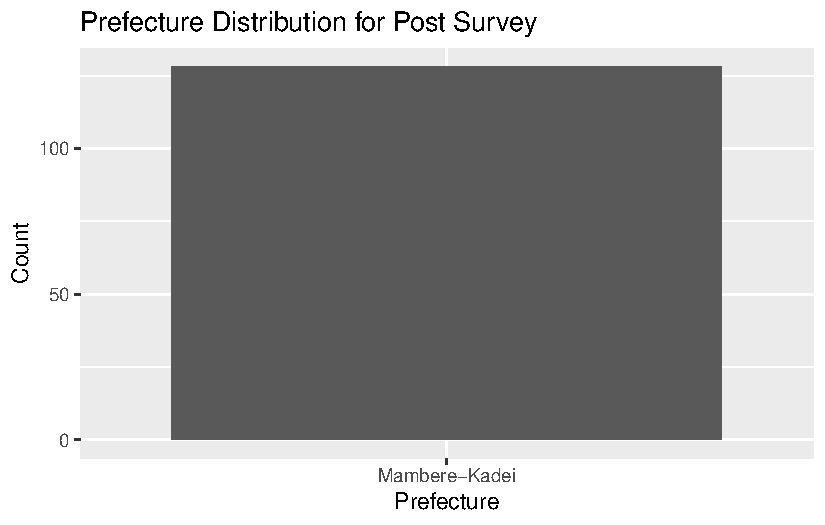
\includegraphics{report_files/figure-pdf/unnamed-chunk-29-1.pdf}

This makes it more clear as the post survey only included residents from
the Mambere-Kadei prefecture, which could be the reason why the
waterpoint site wells differed from the baseline to post.

\hypertarget{map}{%
\paragraph{Map}\label{map}}

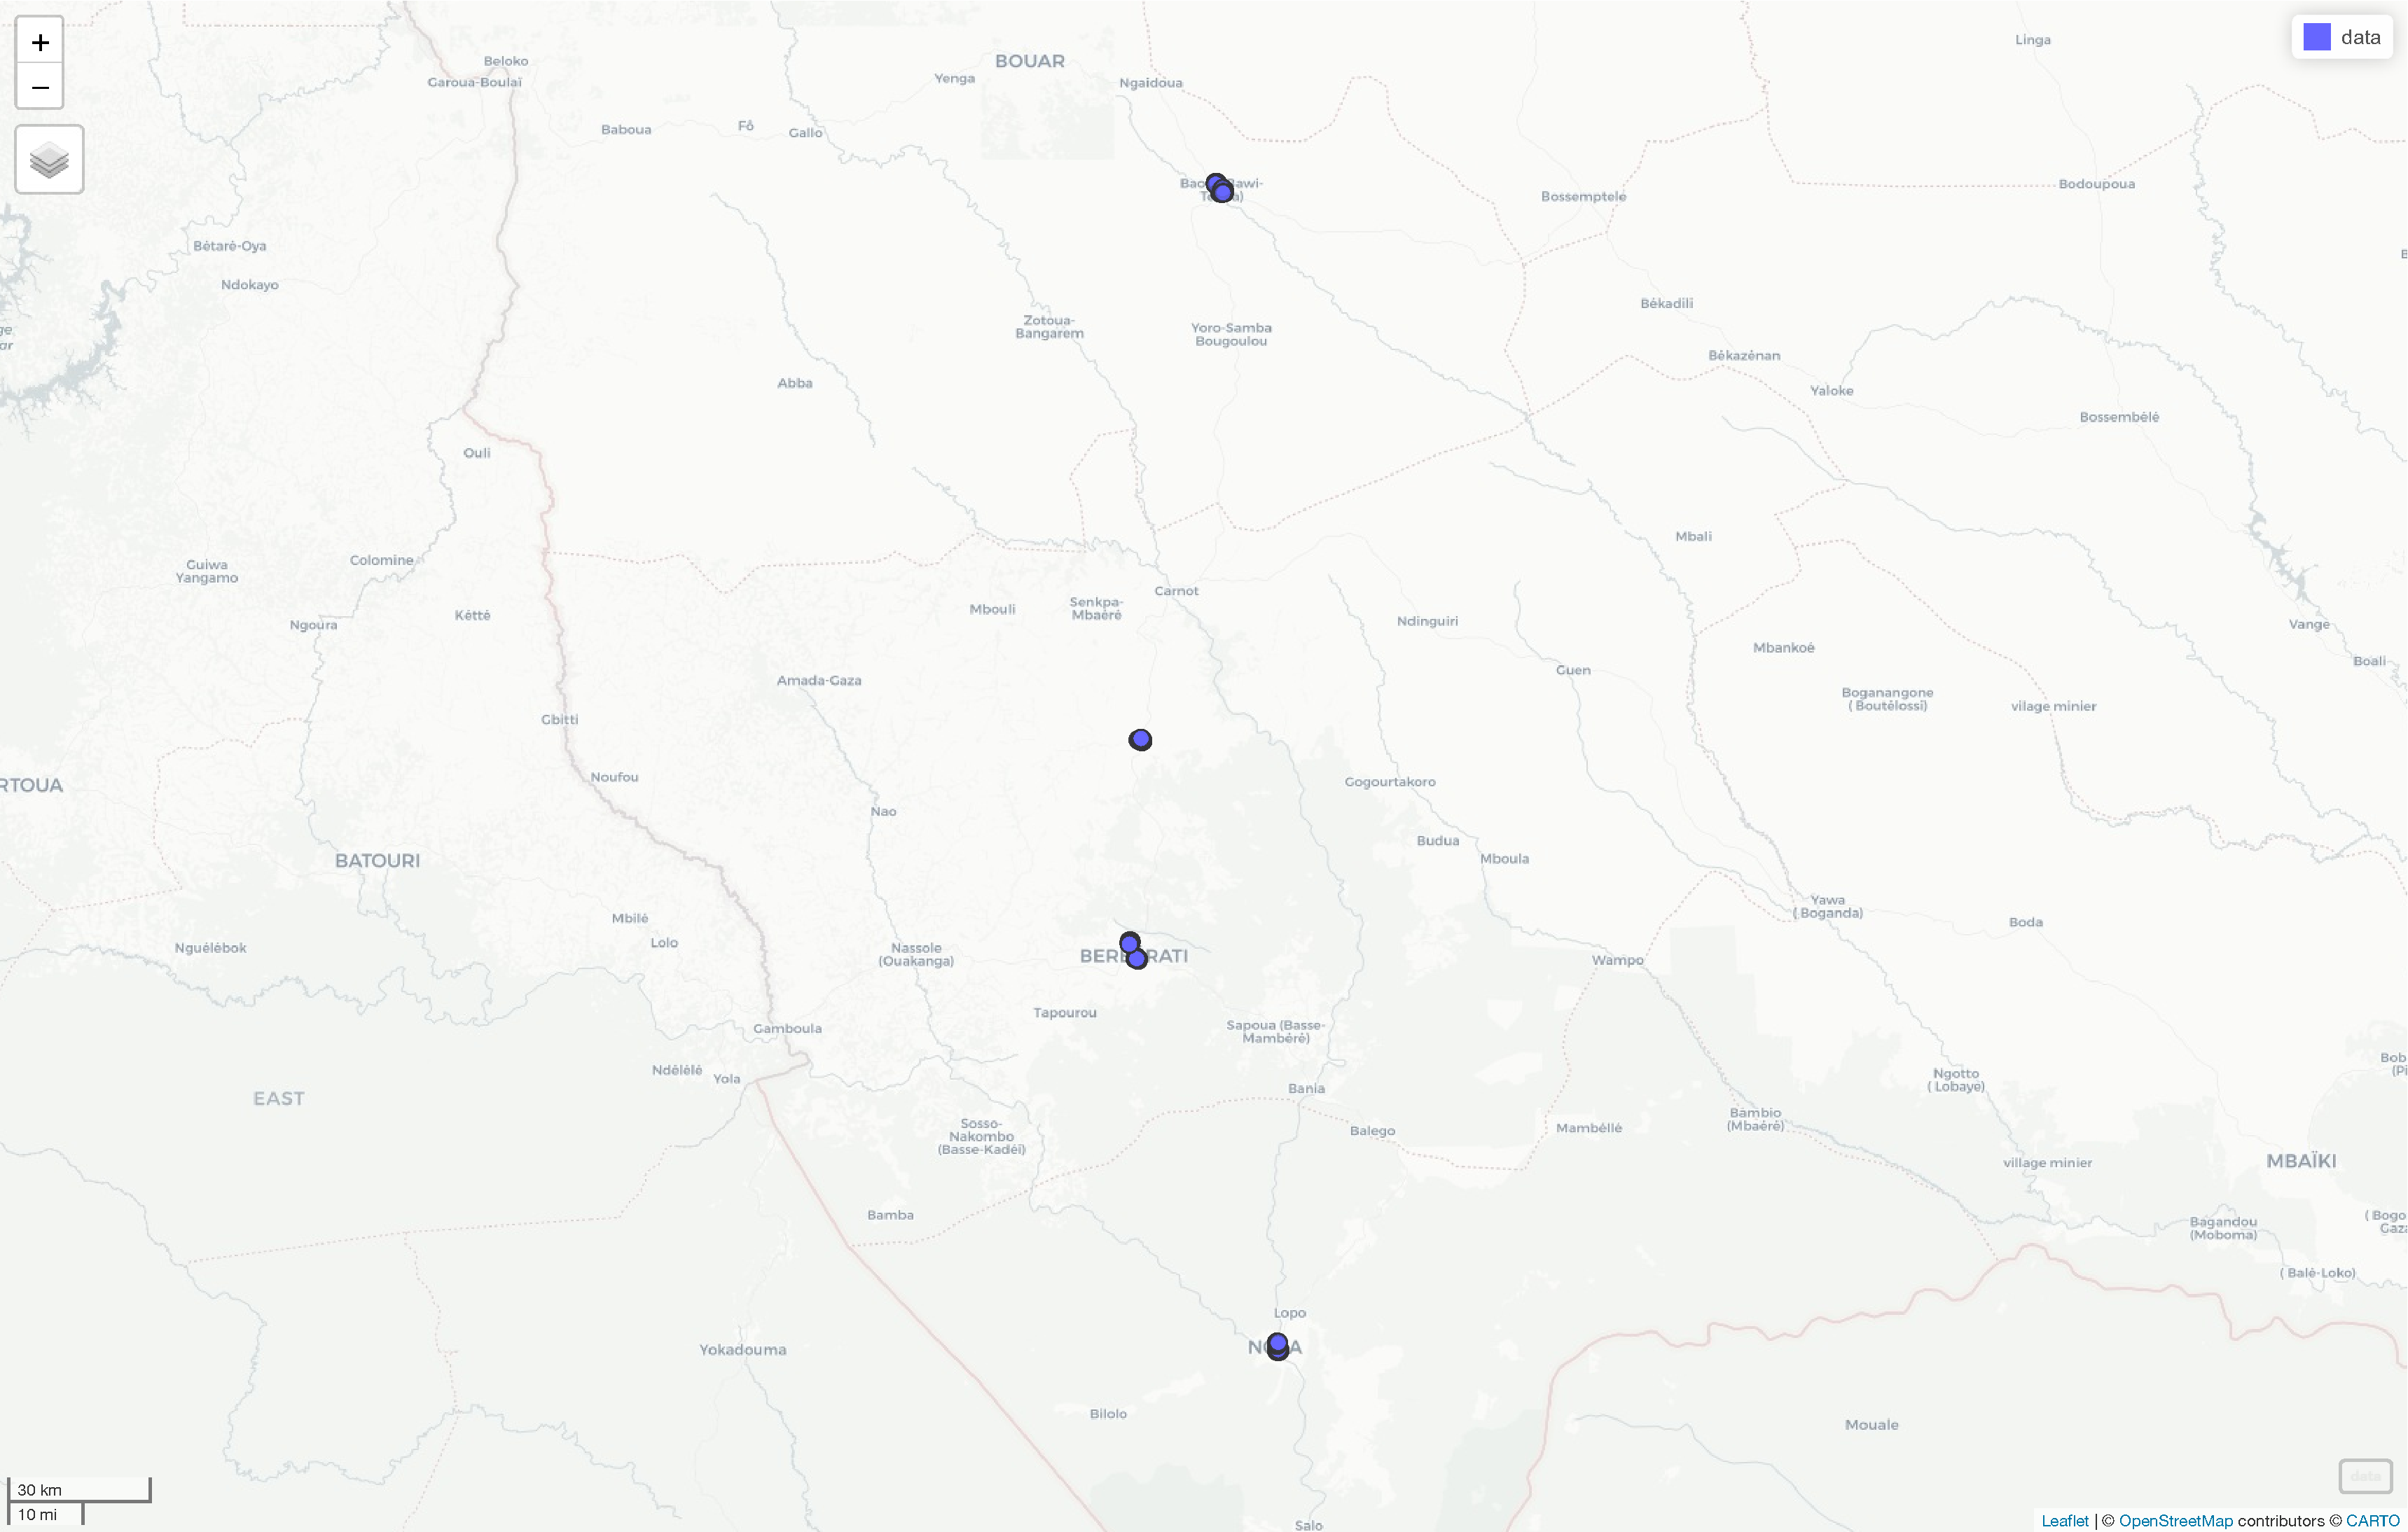
\includegraphics{report_files/figure-pdf/unnamed-chunk-30-1.pdf}

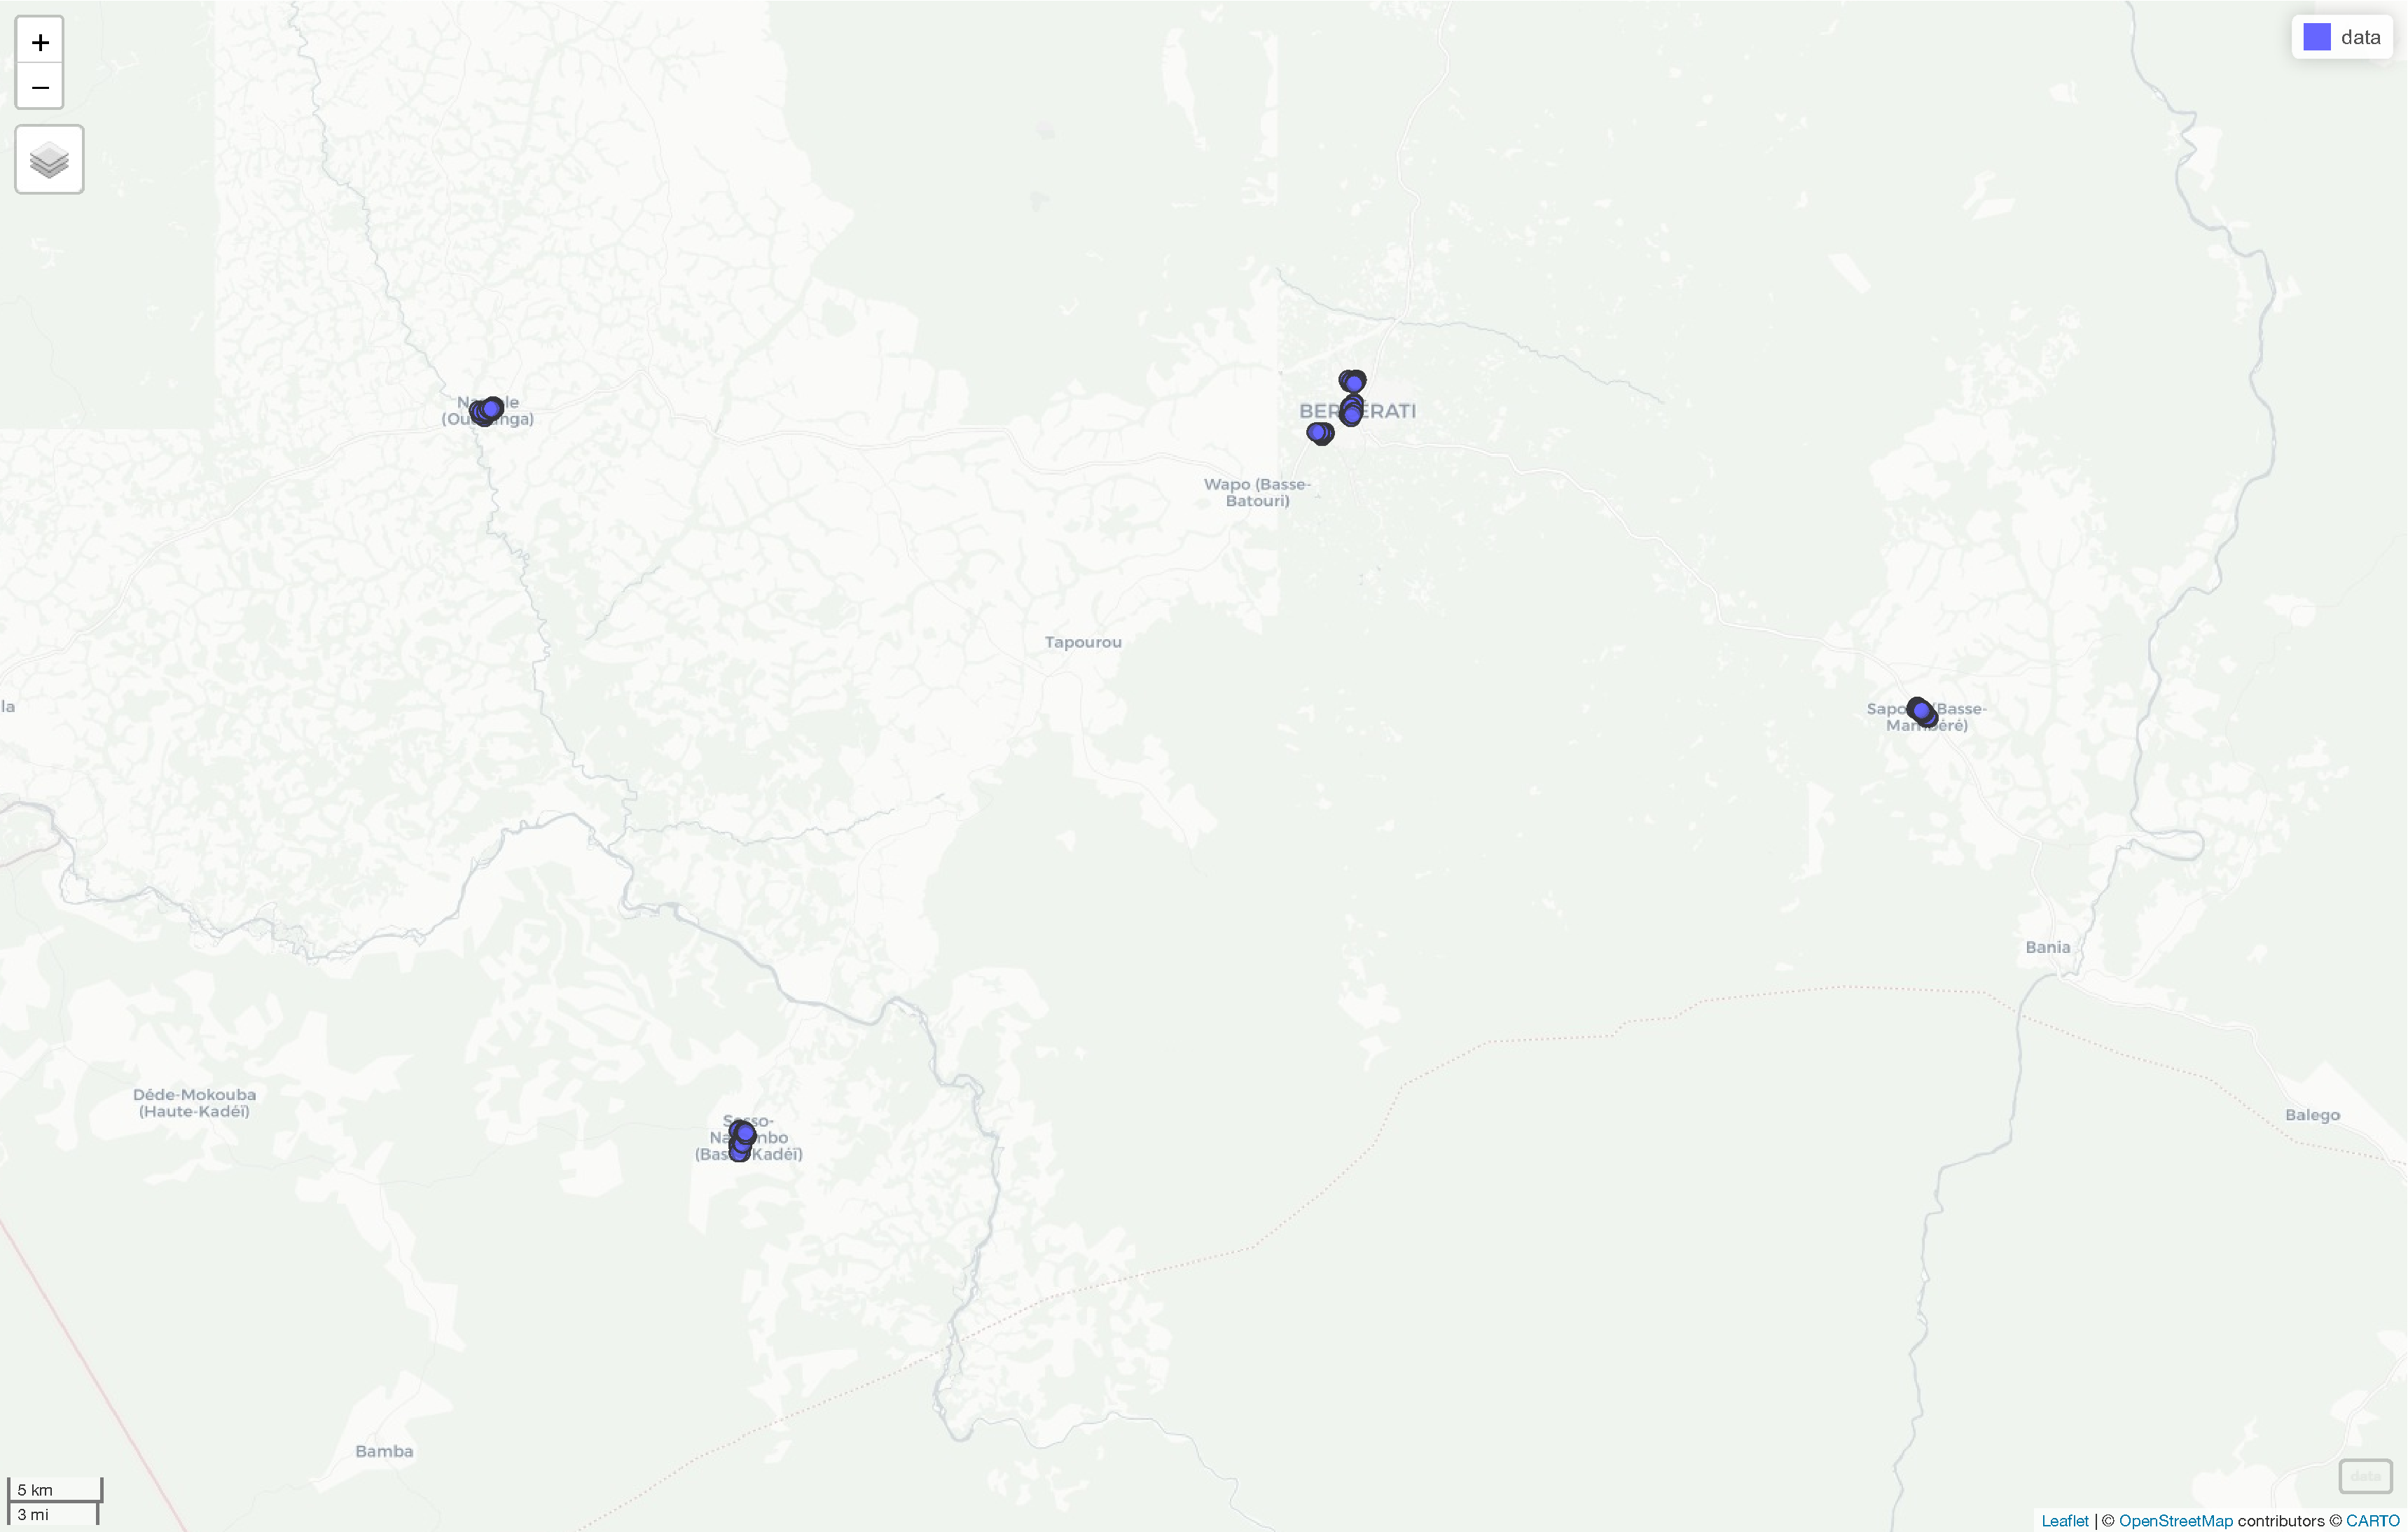
\includegraphics{report_files/figure-pdf/unnamed-chunk-30-2.pdf}

\hypertarget{categorical-answers-to-survey-by-waterpoint-site}{%
\paragraph{Categorical answers to survey by Waterpoint
site}\label{categorical-answers-to-survey-by-waterpoint-site}}

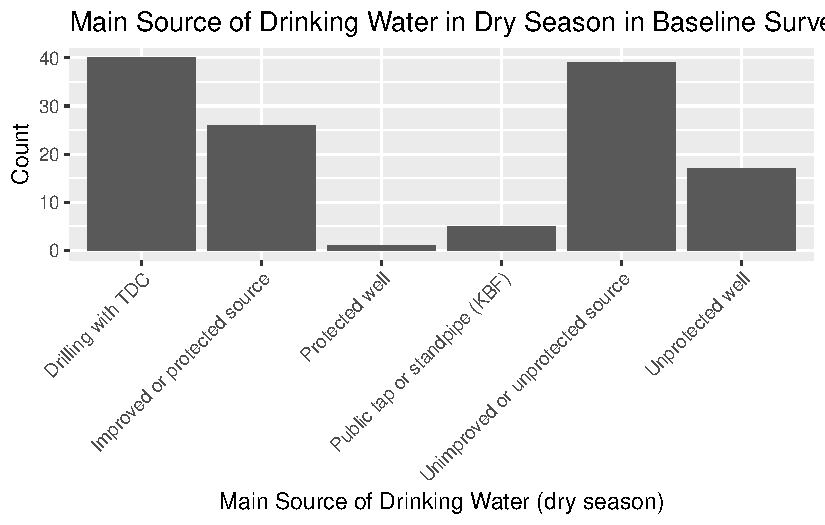
\includegraphics{report_files/figure-pdf/unnamed-chunk-31-1.pdf}

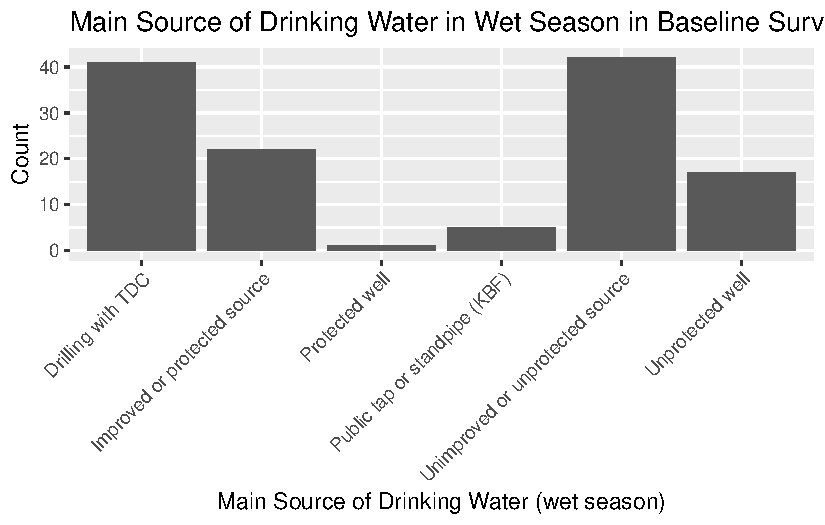
\includegraphics{report_files/figure-pdf/unnamed-chunk-32-1.pdf}

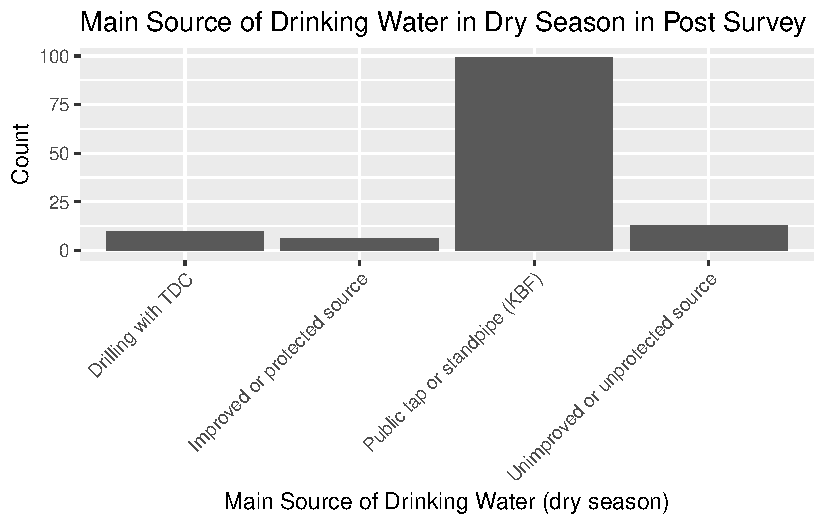
\includegraphics{report_files/figure-pdf/unnamed-chunk-33-1.pdf}

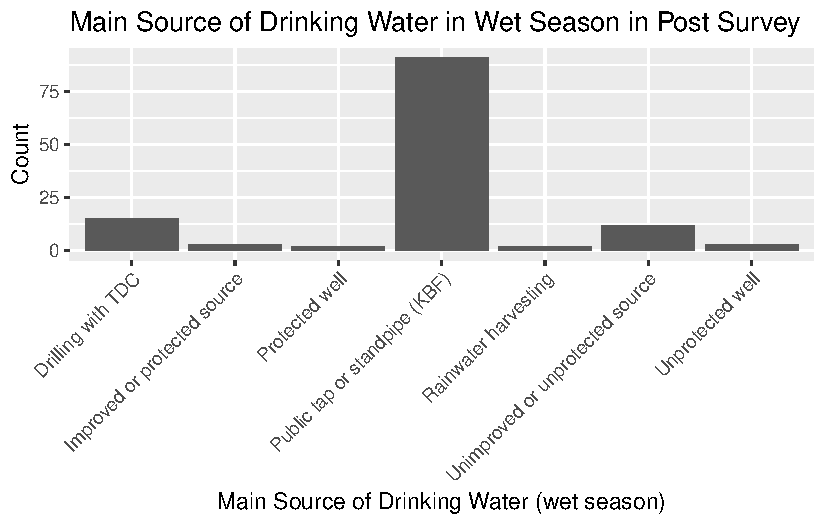
\includegraphics{report_files/figure-pdf/unnamed-chunk-34-1.pdf}

\begin{verbatim}
# A tibble: 10 x 2
   X.Waterpoint.Site.Name count
   <chr>                  <int>
 1 Beautiful View B          13
 2 Dansi C                   12
 3 Dansi F                   13
 4 Karre E                   12
 5 Lomi C                    13
 6 Malebo E                  13
 7 Metezoa E                 13
 8 Nandobo-Center C          13
 9 Nandobo-Centre B          13
10 Sambanda D                13
\end{verbatim}

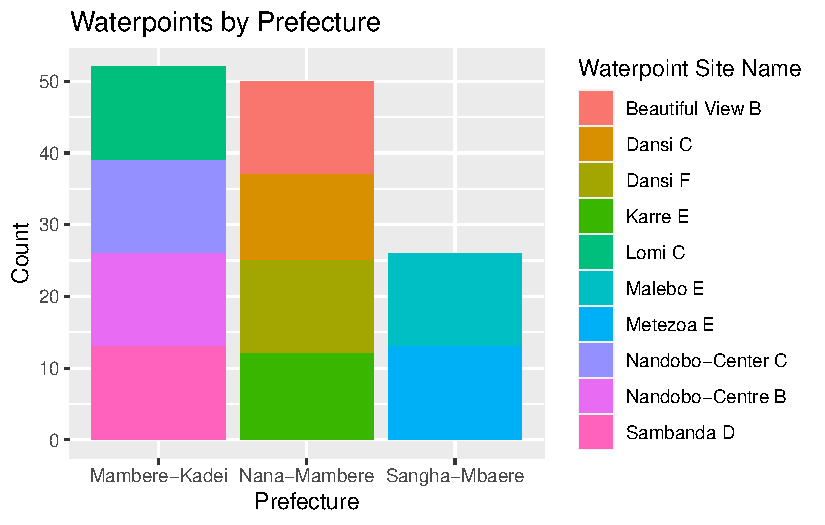
\includegraphics{report_files/figure-pdf/unnamed-chunk-36-1.pdf}



\end{document}
